\documentclass[10pt]{scrbook} \usepackage{modules/nonstahp_book}
\usepackage{mathspec}

\setmainfont[
	Path = f/,
	BoldFont=pb.ttf,
	ItalicFont=pi.ttf,
	BoldItalicFont=pbi.ttf
		]{p.ttf}
\setsansfont[
	Path = f/,
	BoldFont=pb.ttf,
	ItalicFont=pi.ttf,
	BoldItalicFont=pbi.ttf
		]{p.ttf}
		
\setmathfont(Digits)[Path = f/]{p.ttf}
\setmathfont(Latin)[Path = f/]{pi.ttf}
\setmathfont(Greek)[Path = f/, Uppercase]{p.ttf}
\setmathfont(Greek)[Path = f/, Lowercase]{pi.ttf}

\setmonofont[Path = f/]{pmono.ttf}

%\setCJKmainfont[
%	Path=f/,
%	BoldFont=notoserifb.ttf,
%	ItalicFont=notoserifi.ttf,
%	BoldItalicFont=notoserifbi.ttf
%		]{notoserif.ttf}

 \begin{document}

\task{Геометрическая миниатюра}

%\begin{multicols}{2}
\begin{itemize}
\item Как вы думаете, какую часть (по площади) составляет треугольник внутри прямоугольника на картинке ниже?
\begin{center}
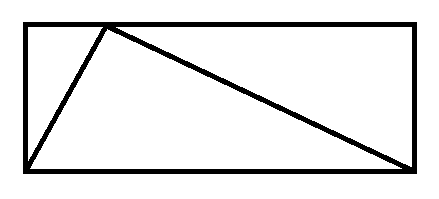
\includegraphics[width=0.7\linewidth]{Area1.png}%1.3
\end{center}
\item А какую часть составляет такой треугольник?
\begin{center}
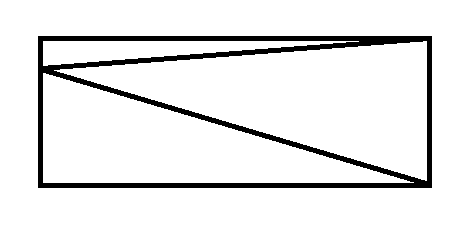
\includegraphics[width=0.7\linewidth]{Area2.png}%1.3
\end{center}
\item Как вы думаете, какую часть (по площади) составляет выделенная область от всего правильного шестиугольника?
\begin{center}
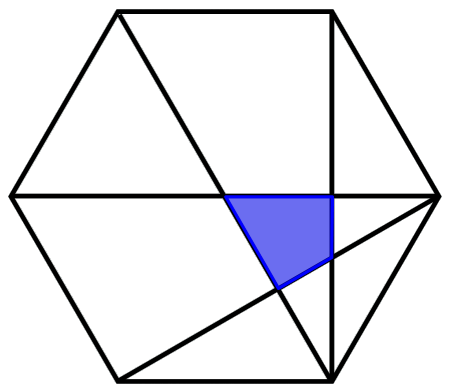
\includegraphics[width=0.7\linewidth]{Area.png}%1.3
\end{center}
\item Выясните, какую часть (по площади) составляет такой треугольник в прямоугольнике
\begin{center}
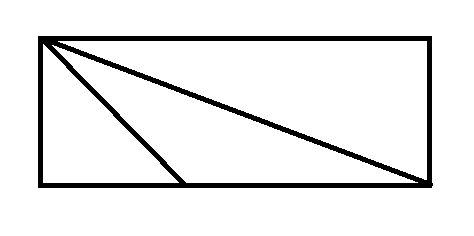
\includegraphics[width=0.7\linewidth]{Area3.png}%1.3
\end{center}
\end{itemize}
%\end{multicols}
















\task{Конфигурации точек}

В 2014 г. на Санкт-Петербургской олимпиаде школьников по математике была предложена следующая задача:
\begin{quote}
На двух параллельных прямых отмечено по 40 точек. Их разбивают на 40 пар так, чтобы отрезки, соединяющие точки в одной паре, не пересекались друг с другом. (В частности, конец одного из отрезков не может лежать на другом отрезке). Докажите, что число способов это сделать не превосходит числа $3^{39}$.
\end{quote}
Последовательность, возникающая в этой задаче, обладает богатыми комбинаторными реализациями, их разнообразие просто изумляет. Опишем общую ситуацию: пусть даны две параллельные прямые, на одной отмечено $k$ точек, на другой $n$ точек. 
\begin{center}
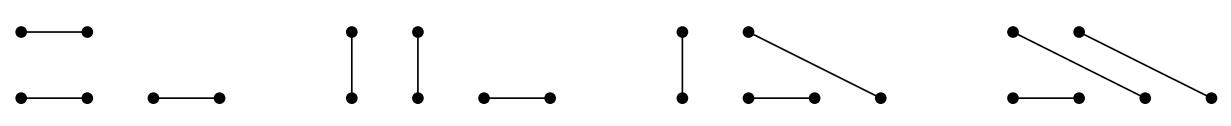
\includegraphics[width=1\linewidth]{Pairs.png}%1.3
\end{center}
Отмеченные точки разбивают на пары так, чтобы отрезки, соединяющие точки в одной паре, не пересекались друг с другом. В частности, конец одного из отрезков не может лежать на другом отрезке. 
\begin{center}
%\begin{figure}[!h]
%\makebox[1 \textwidth][c]{       %centering table
%\resizebox{1 \textwidth}{!}{
\begin{tabular}{c c c c c}
       &       &$[0,0]$&       &     \\
       &$[2,0]$&$[1,1]$&$[0,2]$&     \\
$[4,0]$&$[3,1]$&$[2,2]$&$[1,3]$&$[0,4]$ \\
       &       &$\ldots$&      &
\end{tabular}
%\end{figure}
\end{center}
Полученную картинку будем называть {\itshape конфигурацией} (точек и отрезков на двух прямых) или {\itshape разбиением} (точек на пары). Количество разбиений обозначим через $[k,n]$. Например, $[2,4] = 4$, как показывает рисунок выше.
\begin{center}
%\begin{figure}[!h]
%\makebox[1 \textwidth][c]{       %centering table
%\resizebox{1 \textwidth}{!}{
\begin{tabular}{c c c c c c c c c c c c c c}
 &  &  &  & 1&  &  &  & \\% &       &       &$[0,0]$&       &     \\
 &  &  & 1& 1& 1&  &  & \\ % &       &$[2,0]$&$[1,1]$&$[0,2]$&     \\
 &  & 1& 2&  & 2& 1&  & \\% &$[4,0]$&$[3,1]$&$[2,2]$&$[1,3]$&$[0,4]$ \\
 & 1& 3&  &  &  & 3& 1& \\% &       &       &$\ldots$& & \\
1& 4&  &  &  &  &  & 4& 1%&       &       &$\ldots$& &
\end{tabular}
%\end{figure}
\end{center}
%}
%}
Кроме того, если $n+k$ нечётно, то $[k,n] = 0$, а также $[k,n] = 0$, если $n,k < 0$. Если $n$ или $k$ равно нулю, то $[k,n] = 1$ просто по-определению.
\begin{itemize}
\item Заполните треугольник выше и найдите в нём закономерности, аналогичные закономерностям в треугольнике Паскаля.
\item Выясните, какую последовательность образуют суммы элементов в строках треугольника.
\item Правда ли, что в каждой строчке числа $[k,n]$ обязательно возрастают при движении от краёв к центру?
\item Выясните, как выразить $[n,n]$ через суммы квадратов чисел на диагоналях в треугольнике Паскаля.
\end{itemize}


\end{document}